\section{UTM Services}\label{s:utmServicesTheory}
\paragraph{Idea:} Take the Airbus UTM concept \cite{airbusUTM2018blueprint} combine it with \emph{EUROCONTROL} concept \cite{andrewhately2018} to obtain a legal framework. \emph{Provide conflict resolution functionality} for \emph{Controlled Airspace}:
\begin{enumerate}
    \item \emph{Collision Detection} - define minimal required functionality for collision detection.
    \item \emph{Collision Resolution} - implement \emph{Rules of the Air} \cite{standard1986recommended}.
\end{enumerate}

\begin{figure}[H]
    \centering
    \begin{subfigure}{0.32\textwidth}
        \centering
        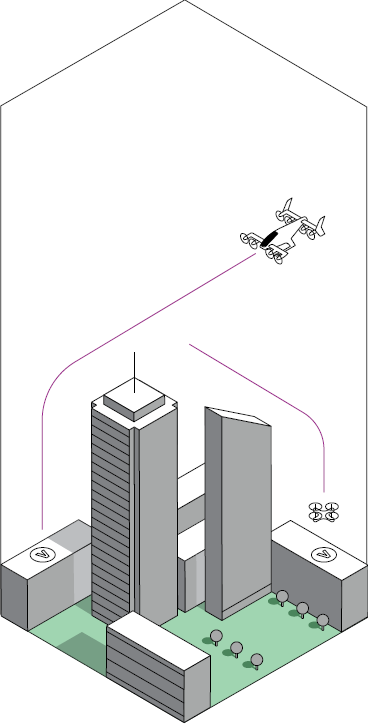
\includegraphics[width=0.9\linewidth]{\FIGDIR/TE032FreeRoute}
        \caption{Free route.}
        \label{fig:UTMFreeRouteMode}
    \end{subfigure}
    \begin{subfigure}{0.32\textwidth}
        \centering
        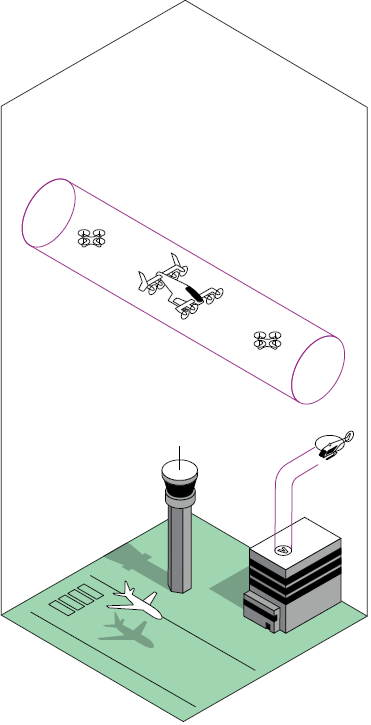
\includegraphics[width=0.9\linewidth]{\FIGDIR/TE034Corridors} 
        \caption{Corridors.}
        \label{fig:CorridorMode}
    \end{subfigure}
    \begin{subfigure}{0.32\textwidth}
        \centering
        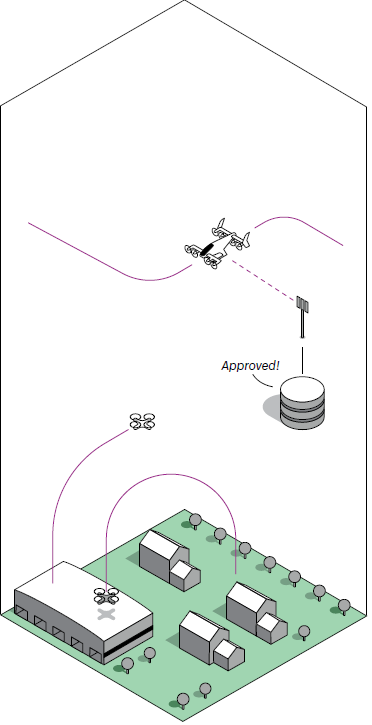
\includegraphics[width=0.9\linewidth]{\FIGDIR/TE035FixedRoute} 
        \caption{Fixed route.}
        \label{fig:fixedRoute}
    \end{subfigure}
    
    \caption{UTM Operation Modes \cite{airbusUTM2018blueprint}.}
    \label{fig:utmOperationModes}
\end{figure}

\paragraph{UTM Operation Modes:} \emph{defined in } \cite{airbusUTM2018blueprint} are following:
\begin{enumerate}
    \item \emph{Free route} (fig. \ref{fig:UTMFreeRouteMode}) is when aircraft can fly any path, so long as their planned path is coordinated with and de-conflicted from the paths of other aircraft by a traffic manager and approved based on calculated risk. Free routing is being introduced worldwide, such as free route airspace. This allows commercial flights to freely plan their route through participating sectors during the cruise. There is less freedom for an aircraft in this situation than in basic flight, since its request may be rejected.
    
    \item\emph{Corridors} (fig. \ref{fig:CorridorMode})  are defined volumes in space, useful for managing airspace in high demand or to manage traffic flow and separation. Coordination is necessary to ensure safety in this airspace. A corridor may take on many different shapes. Aircraft are often guided inside corridors using predetermined routes analogous to approach procedures used worldwide today.
    
    \item\emph{Fixed route} (fig. \ref{fig:fixedRoute}) are used to ensure safety when there is high traffic density or in any location where the structure is required to ensure safe operations. This could include locations such as airports or warehouses. These routes could be constructed or modified dynamically based on calculated risk. The most restrictive version is a predetermined path, where the only variable is when an aircraft is at a specific point in the path.
\end{enumerate}



\paragraph{Used Concepts:} The implementation of our UTM services  is focused on \emph{Free route mode} (fig. \ref{fig:UTMFreeRouteMode}). The \emph{Corridors} and \emph{Fixed routes} are just additional \emph{space/time constraints}.
